\subsection{Concept}

    The unknown of the problem, the boat velocity $\mathbf{u}_b$, is considered in the computation as a boundary condition. In order to determine its value, an iterative process is proposed. 
    The rolling/pitch movement is neglected for now, a "gite" of 15° is considered and only the vertical displacement is allowed in the rigid body motion. 


    \begin{enumerate}
        \item The computation is started with a velocity chosen at random, $U_0 = 3$m/s for instance. 
        \item The drag $\mathbf{D}$ due to water is computed as a postprocessing step after a fully converged M0M1 computation and an average over around 10 flow through times is taken. 
        \item The speed triangle is set to determine the apparent wind, see Fig. \ref{fig:speedtriangle}
        \item The estimation of the thrust applied by the wind $\mathbf{T}$ is detailed in section \ref{section:wind_force}.
        \item The numerically computed drag $\mathbf{D}$ is compared to the estimated thrust $\mathbf{T}$, $\alpha=\frac{||\mathbf{T}||}{||\mathbf{D}||}$.
        \item If $\frac{\alpha_n-\alpha_{n-1}}{\alpha_{n-1}} > 0.01$, the BC is updated $\mathbf{u}_b^{n+1}=\mathbf{u}_b^{n}*\frac{\mathbf{T}}{\mathbf{D}}$ and another computation is launched. 
        \item To prevent overestimation and oscillatory behaviours, a blending factor $r_n$ is used, $\mathbf{u}_b^{n+1}=\mathbf{u}_b^{n}*(1+\alpha r_n(\alpha-1))$. Choosing a low $r_n$ at the beginning and increasing it with $n$ is a good way of proceeding. 
    \end{enumerate}


\subsection{Wind force}
    \label{section:wind_force}
    Two different modes are possible: upwind or downwind. In the former, the sails works as an airfoil with an attached flow, the lift and drag are computed. In the latter, it acts as a planar plate and only the drag of this surface is taken into account (approximated as the product of the sail surface by the stagnation pressure).
    
    In the upwind configuration, lift and drag are computed as follows, with $u$ the scalar product between the apparent wind and a unit vector \textbf{aligned} with the sail:
    \begin{eqnarray}
        F_l = \frac{1}{2}\rho u^2 S C_l, \\ 
        F_d = \frac{1}{2}\rho u^2 S C_d.
        \label{eqn:windforce_upwind}
    \end{eqnarray}

    In the downwind configuration, lift and drag are computed as follows, with $p_s=\frac{1}{2}\rho u^2$, $\alpha=0.5$ a bullshit factor, and $u$ the scalar product between the apparent wind and a unit vector \textbf{perpendicular} to the sail:
    \begin{eqnarray}
        F_l = 0, \\ 
        F_d = \alpha \ S \ p_s.
        \label{eqn:windforce_downwind}
    \end{eqnarray}

    These are expressed in the sail reference frame. The thrust $T$, is the projection of this force on the $x$ axis. 

    In order to determine wether the boat is in upwind or downwind mode (this may change in the iterative algorithm), both modes are computed and the highest thrust value is kept.  

    \begin{figure}[ht!]
        \centering
        \begin{minipage}{0.65\textwidth}
            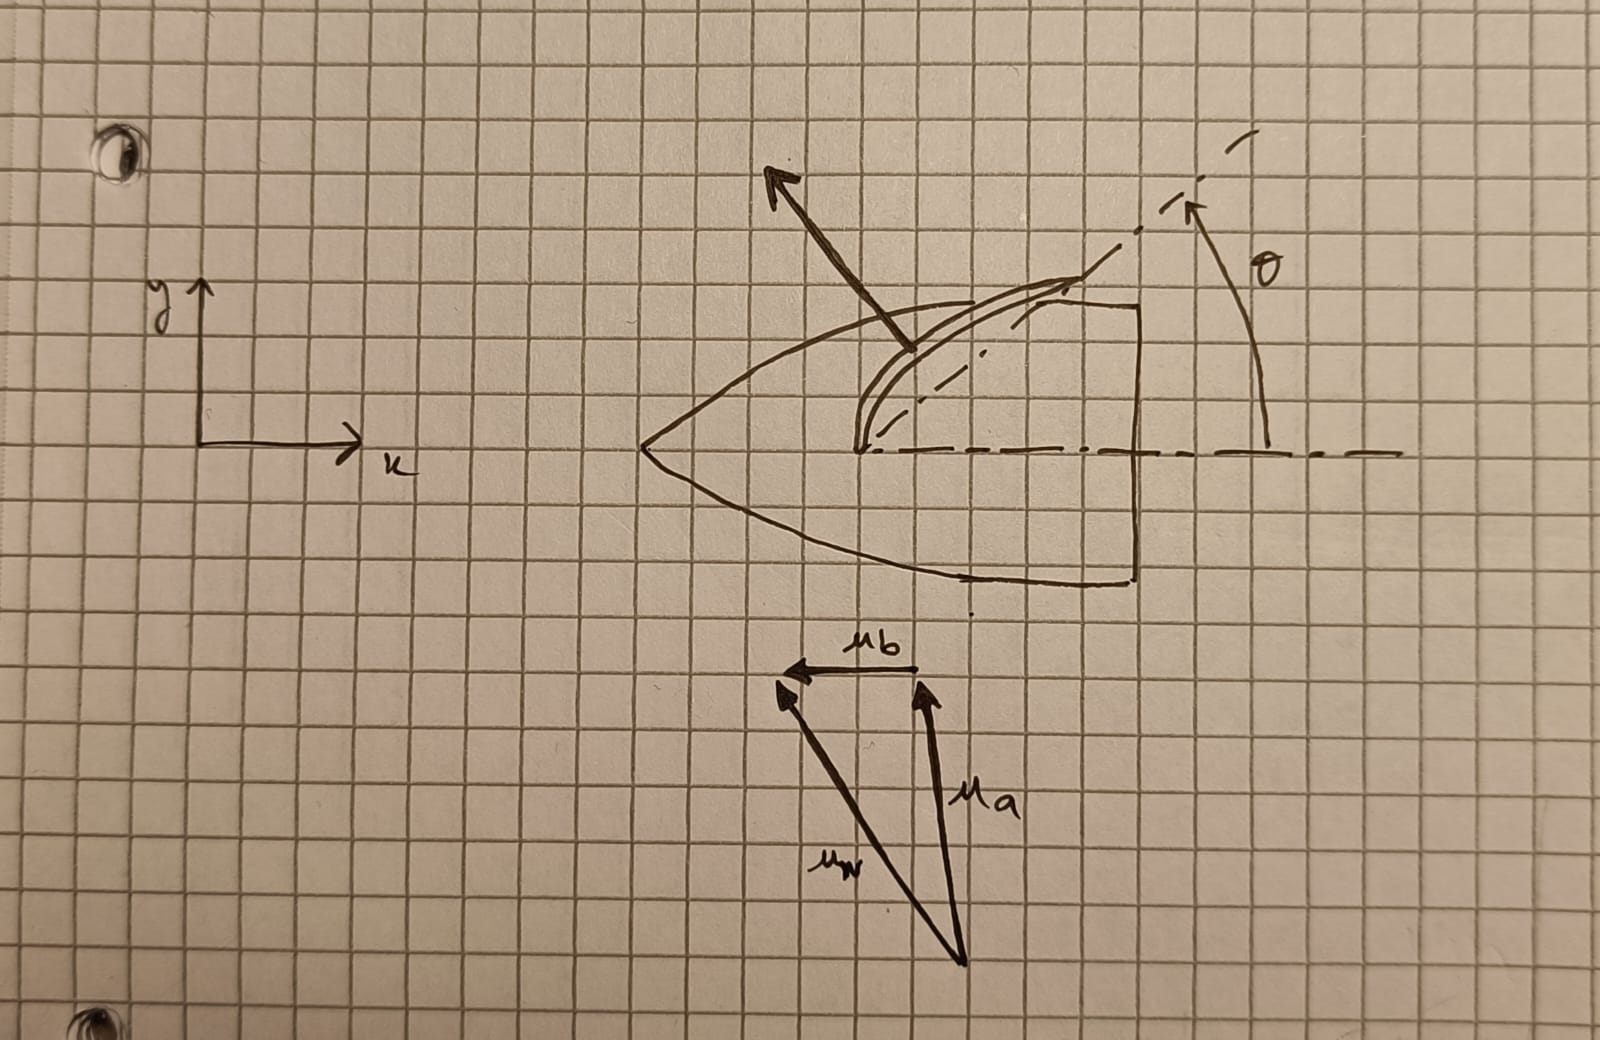
\includegraphics[width=0.99\textwidth]{figures/axes.jpeg}% \\
        \end{minipage}
        \begin{minipage}{0.34\textwidth}
            \vfill
            \begin{tabular}{c|c}
                $\mathbf{u}_w$ & wind speed \\
                $\mathbf{u}_b$ & boat speed \\
                $\mathbf{u}_a$ & apparent wind
            \end{tabular}
            \vfill
        \end{minipage}
        % $U_w$ : wind speed \\
        % $U$ : boat speed \\
        % $U_a$ : apparent wind
        
        \caption{Notations}
        \label{fig:speedtriangle}
    \end{figure}

\clearpage
\subsection{Results}
    \begin{figure}[ht!]
        \centering
        \caption{Iterative determination of the velocity inlet BC for a wind speed of $\langle -10, 10\rangle$ m/s (15  downwind).}
        \label{fig:iterative_process}
    \end{figure}
